%(BEGIN_QUESTION)
% Copyright 2015, Tony R. Kuphaldt, released under the Creative Commons Attribution License (v 1.0)
% This means you may do almost anything with this work of mine, so long as you give me proper credit

Beregn nødvendig verdi for motstanden $R$ i denne kretsen for å begrense strømmen gjennom hver LED til maksimalt 20 milliampere. Anta at fremspenningsfallet for hver LED er 1.7 volt (ved 20 mA):

$$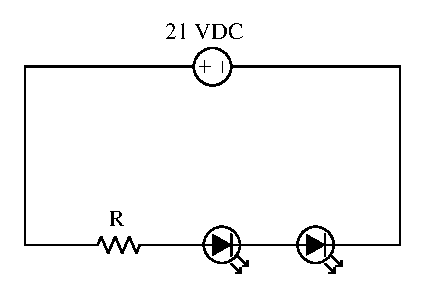
\includegraphics[width=15.5cm]{i00427x01.eps}$$

$R$ = 

\vskip 10pt

Beregn også hvor mye effekt som dissiperes i denne strømbegrensningsmotstanden:

\vskip 10pt

$P_R$ = 

\vskip 10pt

\underbar{file i00427}
%(END_QUESTION)





%(BEGIN_ANSWER)

$R$ = 880 $\Omega$

\vskip 10pt

$P_R$ = 0.352 W

%(END_ANSWER)





%(BEGIN_NOTES)

{\bf Dette spørsmålet er ment for eksamen og ikke for arbeidsark!}.

%(END_NOTES)
